\section{Test results}
 
After performing the described tests we ended up with quite a lot of data. The various test results are summarized in figures, some of which are included further on in this chapter to illustrate interesting and valuable observations.



\begin{figure}[!htb]
	\minipage{0.49\textwidth}
	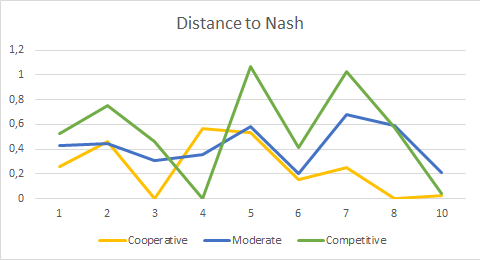
\includegraphics[width=\linewidth]{18_distance_nash}
	\caption{18 Rounds per Opponent}
	\label{fig:18_distance_nash}
	\endminipage\hfill
	\minipage{0.49\textwidth}
	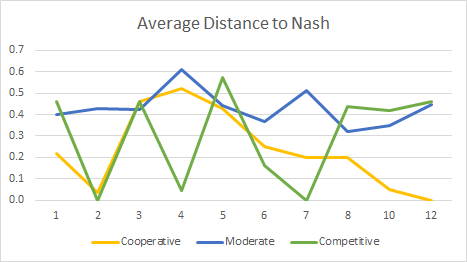
\includegraphics[width=\linewidth]{180_distance_nash}
	\caption{180 Rounds per Opponent}
	\label{fig:180_distance_nash}
	\endminipage\hfill
\end{figure}

Figures \ref{fig:18_distance_nash} and \ref{fig:180_distance_nash} show the average distance to Nash for each set of tournaments



\begin{figure}[!htb]
	\minipage{0.49\textwidth}
	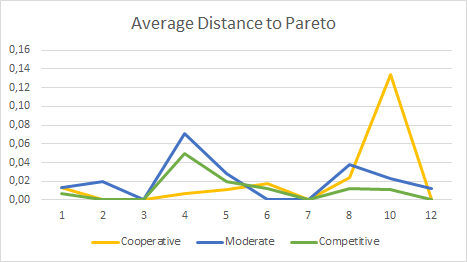
\includegraphics[width=\linewidth]{18_distance_pareto}
	\caption{18 Rounds per Opponent}
	\label{fig:18_distance_pareto}
	\endminipage\hfill
	\minipage{0.49\textwidth}
	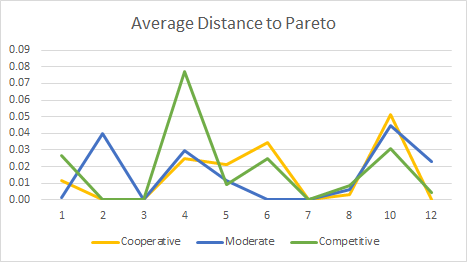
\includegraphics[width=\linewidth]{180_distance_pareto}
	\caption{180 Rounds per Opponent}
	\label{fig:180_distance_pareto}
	\endminipage\hfill
\end{figure}



\begin{figure}[!htb]
	\minipage{0.49\textwidth}
	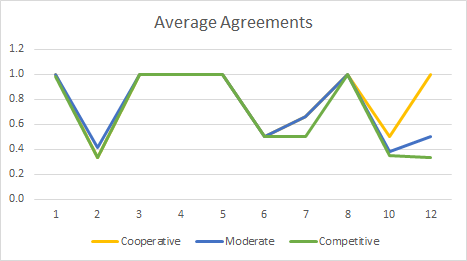
\includegraphics[width=\linewidth]{18_agreements}
	\caption{18 Rounds per Opponent, agreements}
	\label{fig:18_agreements}
	\endminipage\hfill
	\minipage{0.49\textwidth}
	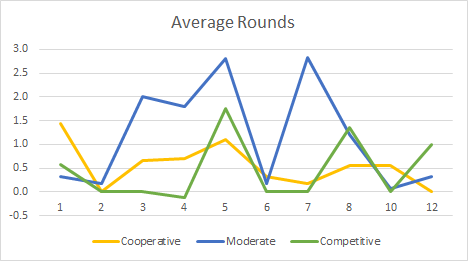
\includegraphics[width=\linewidth]{18_rounds}
	\caption{18 Rounds per Opponent, nr of rounds}
	\label{fig:180_rounds}
	\endminipage\hfill
\end{figure}


\begin{figure}[!htb]
	\minipage{0.49\textwidth}
	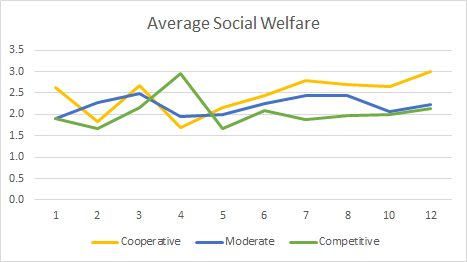
\includegraphics[width=\linewidth]{18_social_welfare}
	\caption{18 Rounds per Opponent}
	\label{fig:18_social_welfare}
	\endminipage\hfill
	\minipage{0.49\textwidth}
	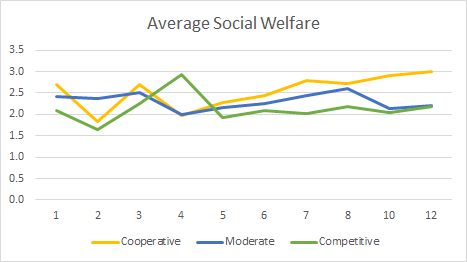
\includegraphics[width=\linewidth]{180_social_welfare}
	\caption{180 Rounds per Opponent}
	\label{fig:180_social_welfare}
	\endminipage\hfill
\end{figure}


\begin{figure}[!htb]
	\minipage{0.49\textwidth}
	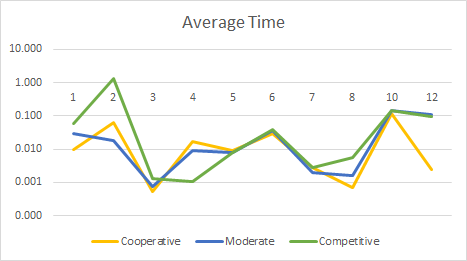
\includegraphics[width=\linewidth]{18_time_log}
	\caption{18 Rounds per Opponent, logarithmic}
	\label{fig:18_time}
	\endminipage\hfill
	\minipage{0.49\textwidth}
	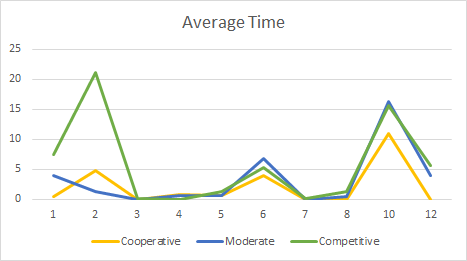
\includegraphics[width=\linewidth]{180_time}
	\caption{180 Rounds per Opponent}
	\label{fig:180_time}
	\endminipage\hfill
\end{figure}



\begin{figure}[!htb]
	\minipage{0.49\textwidth}
	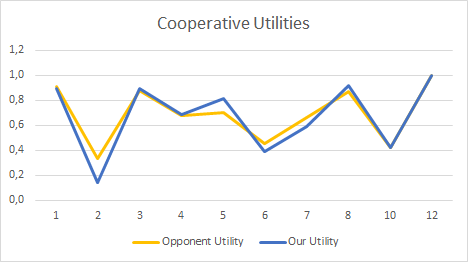
\includegraphics[width=\linewidth]{18_utils_domain_cooperative}
	\caption{18 Rounds per Opponent}
	\label{fig:18_utilscoop}
	\endminipage\hfill
	\minipage{0.49\textwidth}
	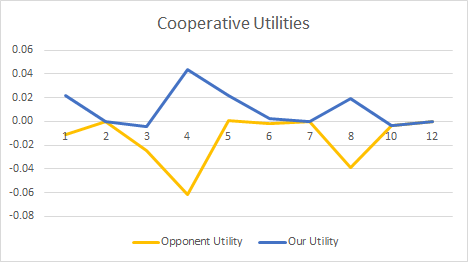
\includegraphics[width=\linewidth]{180_utils_domain_cooperative}
	\caption{180 Rounds per Opponent}
	\label{fig:180_utilscoop}
	\endminipage\hfill
\end{figure}


\begin{figure}[!htb]
	\minipage{0.49\textwidth}
	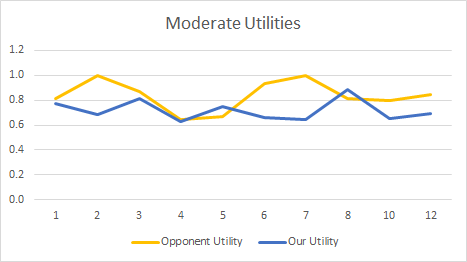
\includegraphics[width=\linewidth]{18_utils_domain_moderate}
	\caption{18 Rounds per Opponent}
	\label{fig:18_utilsmod}
	\endminipage\hfill
	\minipage{0.49\textwidth}
	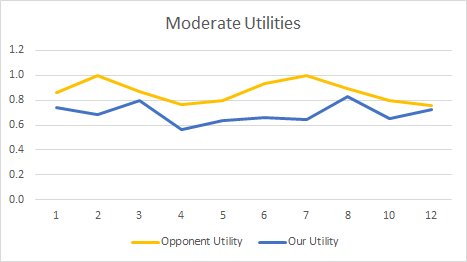
\includegraphics[width=\linewidth]{180_utils_domain_moderate}
	\caption{180 Rounds per Opponent}
	\label{fig:180_utilsmod}
	\endminipage\hfill
\end{figure}


\begin{figure}[!htb]
	\minipage{0.49\textwidth}
	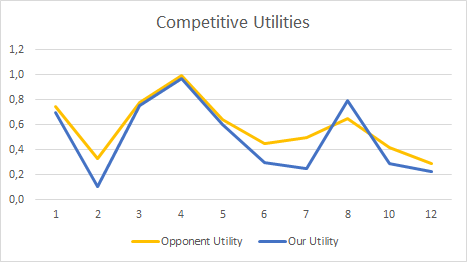
\includegraphics[width=\linewidth]{18_utils_domain_competitive}
	\caption{18 Rounds per Opponent}
	\label{fig:18_utilscomp}
	\endminipage\hfill
	\minipage{0.49\textwidth}
	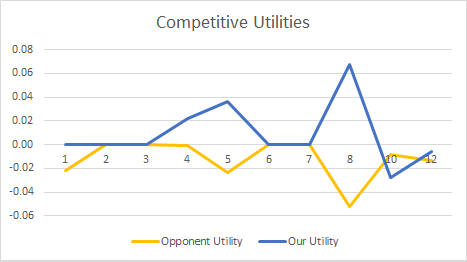
\includegraphics[width=\linewidth]{180_utils_domain_competitive}
	\caption{180 Rounds per Opponent}
	\label{fig:180_utilscomp}
	\endminipage\hfill
\end{figure}






%average distance to nash: cooperate   2 (180) lager
%						 competitive 2+7 (180) lager

%average distance to Pareto: cooperative 10 (18) hoger (domeinspecifiek, gaan we niks mee doen)

%we zien een correlatie tussen meer rounds en lagere agreements (stroevere tegenstander)

%average social welfare is gelijk voor beide

%2 competitive is langzaam

%onze utilities zijn altijd lager dan die van de tegenstander

%competitive utilities: 8 stijgt
%cooperative utilities: 4+5 stijgt
%moderate utilities: 4+5(+8) stijgt